\documentclass[serif, aspectratio=169]{beamer}
%\documentclass[serif]{beamer}  % for 4:3 ratio
\usepackage[T1]{fontenc} 
\usepackage{fourier} % see "http://faq.ktug.org/wiki/uploads/MathFonts.pdf" for other options
\usepackage{hyperref}
\usepackage{latexsym,amsmath,xcolor,multicol,booktabs,calligra}
\usepackage{graphicx,pstricks,listings,stackengine}
\usepackage{lipsum}
\usepackage{xcolor}
\usepackage[english]{babel}
\usepackage[utf8]{inputenc}
\usepackage{graphicx}
\usepackage{array}
\usepackage{ragged2e}
\usepackage{subfigure}
\usepackage{amsmath}
\usepackage{longtable}
\usepackage{etoolbox}
\usepackage{lscape}
\usepackage{algorithm}
\usepackage{algpseudocode}
\usepackage{multirow}
\usepackage{adjustbox}
\usepackage{tabularx}
\usepackage{amsmath,amssymb,amsfonts}
\usepackage{graphicx}
\usepackage{algpseudocode}
\usepackage{textcomp}
\usepackage{mathtools}
\usepackage{adjustbox}
\usepackage{longtable}
\usepackage{multicol}
\usepackage{tabularx}
\usepackage{bibentry}
\usepackage{tikz}
\usetikzlibrary{arrows, positioning, shapes, fit}

% --- THEME SETTINGS START ---
% Since HKUSTstyle is missing, we will simulate a professional academic theme
% similar to the requested style using standard Beamer components.
\usetheme{Madrid}
\usecolortheme{beaver} % A professional red/grey theme often used in academia

% Custom colors to match a university style if needed
\definecolor{uniRed}{RGB}{209, 51, 59}
\definecolor{uniBlue}{RGB}{0, 56, 116}
\definecolor{uniGold}{RGB}{167, 131, 55}

% Customizing blocks to look sharper
\setbeamercolor{block title}{bg=uniRed,fg=white}
\setbeamercolor{block body}{bg=uniRed!10,fg=black}
\setbeamercolor{alertblock title}{bg=uniGold,fg=white}
\setbeamercolor{alertblock body}{bg=uniGold!10,fg=black}

% Font adjustments
\setbeamerfont{title}{size=\Large,series=\bfseries}
\setbeamerfont{subtitle}{size=\large}
% --- THEME SETTINGS END ---

% \setbeamertemplate{bibliography item}{\insertbiblabel}
% \renewcommand{\algorithmicrequire}{\textbf{Input:}}
% \renewcommand{\algorithmicensure}{\textbf{Output:}}

% --- TITLE DETAILS START ---
\author{Scholar Name: Lakshya \texorpdfstring{\\}{, }Registration No.: 25020010001}
\title{Adaptive Gradient Harmonization: Mitigating Modality Dominance}
\subtitle{Unified Representation Learning via Dynamic Convergence Balancing}

\institute{
    Supervisor:  Prof (Dr.) Sandeep Joshi, Department of CSE\\

	%\begin{figure}[htpb]
	%	\begin{center}
	%		\includegraphics[keepaspectratio, scale=0.2]{pic/MUJ.png}
	%	\end{center}
	%\end{figure}
	\textbf{Faculty of Science, Technology and Architecture} \\ 
	\textbf{School of CSE, Department of CSE}\\
	\textbf{Manipal University Jaipur, Rajasthan, India} \\ \vspace{5mm}
	\textbf{January 2026}
}
%\date{\small \today}
%\usepackage{HKUSTstyle} 
% Note: Ensure you have the 'HKUSTstyle.sty' file or comment this line out if not available.

% defs
\def\cmd#1{\texttt{\color{red}\footnotesize $\backslash$#1}}
\def\env#1{\texttt{\color{blue}\footnotesize #1}}


\lstset{
	basicstyle=\ttfamily\small,
	keywordstyle=\bfseries\color{deepblue},
	emphstyle=\ttfamily\color{deepred},    % Custom highlighting style
	stringstyle=\color{deepgreen},
	numbers=left,
	numberstyle=\small\color{halfgray},
	rulesepcolor=\color{red!20!green!20!blue!20},
	frame=shadowbox,
}
% --- TITLE DETAILS END ---

%- --- --- --- --- --- --- --- --- --- --- --- --- --- --- --- 
\begin{document}
\justify
	\begin{frame}
		\titlepage
	\end{frame}
	
	\begin{frame}    
		\tableofcontents[sectionstyle=show,
		subsectionstyle=show/shaded/hide,
		subsubsectionstyle=show/shaded/hide]
	\end{frame}

	% --- 1. Introduction ---
\section{Introduction}
\begin{frame}{Introduction}
    \frametitle<presentation>{Introduction}
    \begin{itemize}
        \item \justifying \textbf{Multimodal Representation Learning}: The field aims to creating unified embeddings that integrate information from diverse sources: Text, Vision, Audio, and Sensors (IMU, Depth, Thermal).
        \item \justifying \textbf{Current State}: Recent "Unified Models" (e.g., ImageBind, Unified-IO 2) can theoretically handle arbitrary input combinations.
        \item \justifying \textbf{The Critical Challenge}: \textbf{Modal Dominance} (or "Modality Laziness").
        \item \justifying Models tend to over-rely on strong signals (RGB Images) and ignore weaker, noisier signals (Audio/Sensors), leading to poor robustness when the dominant modality is missing.
    \end{itemize}
\end{frame}

% --- 2. Problem Statement ---
\section{Problem Statement}
\begin{frame}{Problem Statement}
    \frametitle<presentation>{Problem Statement}
    This research addresses the \textbf{misalignment of convergence rates} and \textbf{gradient dominance} in unified multimodal learning.
    \vspace{0.5cm}
    \begin{itemize}
        \item \textbf{Modality Laziness}: High-SNR modalities (Vision) dominate the joint optimization, suppressing learning from weaker ones.
        \item \textbf{Lack of Robustness}: "Unified" representations fail to generalize when key sensors fail or dominant modalities are corrupted.
        \item \textbf{Static Optimization}: Current methods use manual/static loss weighting, which is brittle and fails to adapt to training dynamics.
    \end{itemize}
\end{frame}

% --- 3. Literature Review ---
\section{Literature Review}

% Part 1: Foundational Papers (BACD Framework)
\begin{frame}{}
    \frametitle<presentation>{Literature Review - Part 1: Foundational Papers}
\tiny{
\begin{table}
    \caption{Summary of Foundational Papers (BACD Framework)}	
    \label{tab:litreview-foundational} 

    \begin{tabularx}{\textwidth}{p{2.0cm}p{2.5cm}p{3.5cm}p{3.5cm}} 
        \toprule
        \textbf{Paper} & \textbf{Core Concept} & \textbf{Key Contribution} & \textbf{Identified Gap} \\ 		
        \midrule

        \textbf{Gradient Blending} (Wang et al., CVPR 2020) &
        Overfitting-based gradient weighting for multimodal fusion. &
        First systematic analysis: multimodal networks underperform due to dominant modality overfitting. 400+ citations. &
        Static/periodic updates; not real-time adaptive. \\ \hline

        \textbf{Greedy Nature} (Wu et al., ICML 2022) &
        Coined "Modality Laziness"; proved it hurts generalization. &
        Conditional Learning Speed (CLS) metric to quantify and balance modality learning rates. 181 citations. &
        CLS metric is complex to compute; requires extensive calibration. \\ \hline

        \textbf{OGM-GE} (Peng et al., CVPR 2022 Oral) &
        On-the-fly gradient modulation with generalization enhancement. &
        Dynamic noise injection to slow dominant modality. Proven at CVPR Oral (top 5\%). 100+ citations. &
        Noise injection is a "black box"; lacks interpretability. \\ \hline

        \textbf{Cross-Modality Harmonization} (Google, NeurIPS 2022) &
        Gradient conflict resolution at billion-sample scale. &
        Gradient realignment and curriculum learning based on conflict signals. Deployed at Google scale. &
        Designed for massive scale; heavy computational cost for smaller benchmarks. \\

        \noalign{\smallskip}\hline
    \end{tabularx}
\end{table}}
\end{frame}

% Part 2: Recent SOTA Models (2023-2024)
\begin{frame}{}
    \frametitle<presentation>{Literature Review - Part 2: Recent SOTA Models}
\tiny{
\begin{table}
    \caption{Summary of Recent State-of-the-Art Multimodal Models (2023-2024)}	
    \label{tab:litreview-sota} 

    \begin{tabularx}{\textwidth}{p{2.0cm}p{2.5cm}p{3.5cm}p{3.5cm}} 
        \toprule
        \textbf{Paper} & \textbf{Core Concept} & \textbf{Key Contribution} & \textbf{Identified Gap} \\ 		
        \midrule

        \textbf{ImageBind} (Girdhar et al., CVPR 2023) &
        Joint embedding across 6 modalities (Image, Text, Audio, Depth, Thermal, IMU). &
        Zero-shot alignment using Images as the "binding" glue. No need for $O(N^2)$ paired data. &
        Heavily reliant on paired image data stability. prone to visual bias. \\ \hline

        \textbf{Unified-IO 2} (Lu et al., 2023) &
        Autoregressive transformer for generation \& understanding. &
        Massive scale (7B params), handles diverse tasks (GRIT SOTA). &
        High computational cost; does not explicitly solve gradient suppression of weak signals. \\ \hline

        \textbf{Meta-Transformer} (Zhang et al., 2023) &
        Frozen encoder framework for 12 modalities. &
        Decouples perception from semantic understanding using a shared token space. &
        Relies on frozen backbones; limited adaptation to novel, noisy sensor noise profiles. \\ \hline

        \textbf{Deep Multimodal Learning Survey} (Wu et al., 2024) &
        Review of Missing Modality techniques. &
        Categorizes approaches into Data Augmentation, Robust Fusion, and Learning-based methods. &
        Highlights lack of "parameter-free" adaptive optimization for sensor fairness. \\

        \noalign{\smallskip}\hline
    \end{tabularx}
\end{table}}
\end{frame}

% Part 3: Datasets
\begin{frame}{}
    \frametitle<presentation>{Literature Review - Part 3: Datasets Used}
    
    \begin{columns}[T]
        % Column 1: CIFAR-10
        \begin{column}{0.48\textwidth}
            \begin{block}{CIFAR-10 (Vision - Dominant)}
                \small
                \begin{itemize}
                    \item 60,000 color images (32×32 pixels)
                    \item 10 classes: airplane, automobile, bird, cat, deer, dog, frog, horse, ship, truck
                    \item \textbf{Role}: Dominant Modality
                    \item High SNR → easy for CNNs
                    \item Models reach \textgreater90\% accuracy quickly
                    \item \textcolor{red}{\textbf{Problem}}: Causes model to ignore audio
                \end{itemize}
            \end{block}
        \end{column}
        
        % Column 2: CREMA-D
        \begin{column}{0.48\textwidth}
            \begin{block}{CREMA-D (Audio - Weak)}
                \small
                \begin{itemize}
                    \item 7,442 emotion audio clips
                    \item 91 actors (diverse demographics)
                    \item 6 emotions: Anger, Disgust, Fear, Happiness, Neutral, Sadness
                    \item \textbf{Role}: Weak/Lazy Modality
                    \item Temporally complex, noisy
                    \item Slower to learn than visual patterns
                \end{itemize}
            \end{block}
        \end{column}
    \end{columns}
    
    \vspace{0.3cm}
    
    \begin{alertblock}{The "High-Imbalance" Protocol}
        \small
        \textbf{Challenge}: By pairing CIFAR-10 (easy) + CREMA-D (hard), we create a controlled experiment that reliably reproduces \textbf{Modality Laziness}. The optimizer naturally gravitates toward CIFAR-10 gradients, forcing our MFC to actively balance learning.
    \end{alertblock}
\end{frame}

% --- 4. Objectives ---
\section{Objective}
\begin{frame}{Objective}
    \frametitle<presentation>{Research Objectives}
    \begin{itemize}
        \item \justifying \textbf{To Develop}: An \textbf{Adaptive Gradient Harmonization} algorithm ("Modality Fairness Controller") that dynamically re-weights loss components based on real-time generalization rates.
        \item \justifying \textbf{To Implement}: A \textbf{Dynamic Convergence Balancing} mechanism ensuring weak modalities (Audio/Sensors) reach optimal representation power alongside strong ones (Vision).
        \item \justifying \textbf{To Evaluate}: Rigorous testing on standard benchmarks (e.g., AudioSet, COCO) and robustness scenarios (inference with missing dominant modalities).
    \end{itemize}
\end{frame}

% --- 5. Methodology ---
\section{Methodology}
\begin{frame}{Proposed Methodology: The "Modality Fairness Controller"}
    \textbf{Core Concept:}
    \begin{itemize}
        \item Replaces static weights with dynamic scalars $\lambda_m(t)$.
        \item Monitors \textbf{Overfitting-to-Generalization Ratio (OGR)}.
    \end{itemize}
    \vspace{0.5cm}
    \textbf{Mechanism:}
    \begin{itemize}
        \item \textbf{Throttle}: If Vision learns too fast ($\Delta L_v \gg$), reduce $\lambda_{vision}$.
        \item \textbf{Amplify}: If Audio lags, increase $\lambda_{audio}$ to force feature extraction.
    \end{itemize}
\end{frame}

\begin{frame}{Proposed Methodology: System Architecture}
    \centering
    \resizebox{0.85\textwidth}{!}{%
    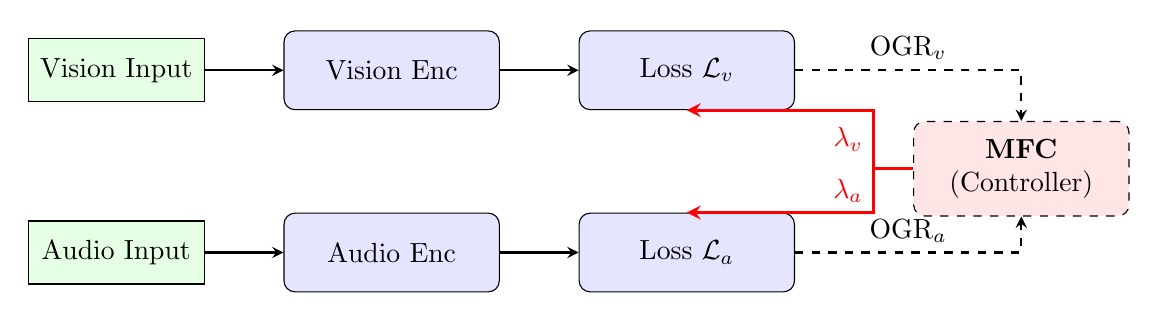
\begin{tikzpicture}[node distance=1.2cm, >=stealth, auto,
        block/.style={rectangle, draw, fill=blue!10, text width=2.5cm, text centered, rounded corners, minimum height=1.0cm},
        sensor/.style={rectangle, draw, fill=green!10, text width=2.0cm, text centered, minimum height=0.8cm},
        control/.style={rectangle, draw, fill=red!10, text width=2.5cm, text centered, rounded corners, minimum height=1.2cm, dashed}
        ]
        % Nodes
        \node [sensor] (vis) {Vision Input};
        \node [block, right=1cm of vis] (encv) {Vision Enc};
        \node [block, right=1cm of encv] (lossv) {Loss $\mathcal{L}_v$};

        \node [sensor, below=1.5cm of vis] (aud) {Audio Input};
        \node [block, right=1cm of aud] (enca) {Audio Enc};
        \node [block, right=1cm of enca] (lossa) {Loss $\mathcal{L}_a$};
        
        \node [control, right=1.5cm of lossv, yshift=-1.25cm] (mfc) {\textbf{MFC} \\ (Controller)};
        
        % Edges
        \draw[->, thick] (vis) -- (encv);
        \draw[->, thick] (encv) -- (lossv);
        
        \draw[->, thick] (aud) -- (enca);
        \draw[->, thick] (enca) -- (lossa);
        
        % Feedback
        \draw[->, dashed, thick] (lossv) -| node[near start, above] {OGR$_v$} (mfc);
        \draw[->, dashed, thick] (lossa) -| node[near start, above] {OGR$_a$} (mfc);
        
        \draw[->, red, very thick] (mfc.west) -- ++(-0.5,0) |- node[near start, left] {$\lambda_v$} (lossv.south);
        \draw[->, red, very thick] (mfc.west) -- ++(-0.5,0) |- node[near start, left] {$\lambda_a$} (lossa.north);
        
    \end{tikzpicture}
    }
    \begin{figure}
    \caption{Adaptive Training Loop: The MFC monitors OGR and dynamically scales loss weights ($\lambda$) to balance convergence.}
    \end{figure}
\end{frame}

% --- 6. Proposed Contributions ---
\section{Proposed Contributions}
\begin{frame}{Research Contributions}
    \frametitle<presentation>{Key Contributions}
    \begin{itemize}
        \item \justifying \textbf{Taxonomy}: A structured classification of "Modality Laziness" phenomena in current unified models.
        \item \justifying \textbf{Algorithm}: The \textbf{Adaptive Gradient Harmonization} method, a parameter-free approach to balancing heterogeneous sensor fusion.
        \item \justifying \textbf{Framework}: A Unified Transformer architecture integrated with the fairness controller, capable of robust performance even with missing data.
        \item \justifying \textbf{Benchmark}: Evaluation on modern multimodal datasets comparisons against static weighting baselines (ImageBind, Meta-Transformer).
    \end{itemize}
\end{frame}

% --- 7. Schedule / Progress ---
\section{Work Done \& Schedule}
\begin{frame}{Work Done (First 6 Months)}
    \frametitle<presentation>{Status Update}
    \begin{itemize}
        \item \textbf{Phase 1: Literature Survey (Completed)} 
        \begin{itemize}
            \item Reviewed key papers: ImageBind, Unified-IO 2, Meta-Transformer.
            \item Analyzed gaps in "Missing Modality" research (Wu et al. 2024).
        \end{itemize}
        \item \textbf{Phase 2: Problem Formulation (Completed)}
        \begin{itemize}
            \item Defined "Modality Laziness" as the core optimization bottleneck.
            \item Formulated the hypothesis for Dynamic Convergence Balancing.
        \end{itemize}
        \item \textbf{Phase 3: Resource Collection (Ongoing)}
        \begin{itemize}
             \item Acquired datasets (AudioSet, COCO) and baseline codebases.
        \end{itemize}
    \end{itemize}
\end{frame}

\begin{frame}{Future Plan}
    \frametitle<presentation>{Schedule (Next 6 Months)}
    \begin{figure}
        \centering
        % \includegraphics[width=0.8\linewidth]{Schedule.jpg}
        \begin{tabular}{|l|l|l|}
        \hline
        \textbf{Month} & \textbf{Activity} & \textbf{Outcome} \\ \hline
        Month 7-8 & Implementation of Baseline & Functional Unified Transformer \\ \hline
        Month 9-10 & Develop "Fairness Controller" & Working Adaptive Algorithm \\ \hline
        Month 11-12 & Evaluation \& Thesis Writing & Comparative Results \& First Draft \\ \hline
        \end{tabular}
        \caption{Project Timeline}
    \end{figure}
\end{frame}

% --- 8. Conclusion ---
\section{Conclusion}
\begin{frame}{Conclusion}
    \frametitle<presentation>{Conclusion}
    \begin{itemize}
        \item \justifying Current Multimodal models suffer from \textbf{Modality Laziness}, where strong visual signals suppress learning from audio/sensors.
        \item \justifying We propose a novel \textbf{Adaptive Gradient Harmonization} approach to dynamically balance learning rates across modalities.
        \item \justifying By forcing the model to learn "fairly", we aim to achieve \textbf{true unified robustness}, ensuring performance holds even when dominant sensors fail.
    \end{itemize}
\end{frame}

% --- References ---
\section*{References}
\begin{frame}[allowframebreaks]
    \frametitle<presentation>{Selected References}
    \footnotesize
    \begin{thebibliography}{99}
        % Core BACD Framework Papers (Foundational)
        \bibitem{gradientblending} Wang, W., et al. "What Makes Training Multi-Modal Classification Networks Hard?" \textit{CVPR}, 2020. (400+ citations)
        \bibitem{greedynature} Wu, Y., et al. "Characterizing and Overcoming the Greedy Nature of Learning in Multi-modal Deep Neural Networks." \textit{ICML}, 2022. (181 citations)
        \bibitem{ogmge} Peng, Y., et al. "Balanced Multimodal Learning via On-the-fly Gradient Modulation." \textit{CVPR}, 2022 Oral. (100+ citations)
        \bibitem{crossmodality} Google Research. "Scaling Multimodal Pre-Training via Cross-Modality Gradient Harmonization." \textit{NeurIPS}, 2022.
        
        % SOTA Literature Review Papers (2023-2024)
        \bibitem{imagebind} Girdhar, R., et al. "ImageBind: One Embedding Space To Bind Them All." \textit{CVPR}, 2023.
        \bibitem{unifiedio2} Lu, J., et al. "Unified-IO 2: Scaling Autoregressive Multimodal Models with Vision, Language, Audio, and Action." \textit{arXiv}, 2023.
        \bibitem{metatransformer} Zhang, Y., et al. "Meta-Transformer: A Unified Framework for Multimodal Learning." \textit{arXiv}, 2023.
        \bibitem{missingmodality} Wu, R., et al. "Deep Multimodal Learning with Missing Modality: A Survey." \textit{ACM Computing Surveys}, 2024.
    \end{thebibliography}
\end{frame}

% --- Thank You ---
\begin{frame}
    \centering
    \vspace{1cm}
    \Huge \textbf{Thank You}
    \vspace{0.5cm}
    \Large \\ Questions?
\end{frame}
	
\end{document}
